\chapter{ConFs File System}
\label{chapter:ConFs}

\section{Overview}
To test the capabilities of ConFrm, we implemented ConFs, a confidential, crash-safe file system with a checksum based and encrypted log. 
ConFs is a crash-safe file system implemented in Coq and its confidentiality is proven using ConFrm framework. It has a checksum based and encrypted log, a log cache for faster log reads, a transaction system for atomic operations, two block allocators for managing data and inode blocks, and an authentication system for access control. All these components are implemented on top of each other and intermediate abstraction layers are used to provide a cleaner interface for the components above.

\section{Implementation}
We implemented ConFs as a stack of levels, each level consisting of a ConFrm layer and the programs written in that layer. This approach allows us to simplify the operational semantics as we implement higher level functionality. Each layer is designed to model how underlying implementation and hardware behaves. Using ConFrm's layer structure allow us to use the machinery and the meta-theory provided. This allowed us to encapsulate different parts of the system to only the relevant state and operations, reducing the proof effort significantly.

In the case of a layer abstracting an implementation from the level below, a simulation proof is employed to ensure that layer's semantics captures the behavior of the implementation. We will explain each level, starting from the bottom, in the following part. Figure \ref{fig:ConFs_Layers} shows how different parts of ConFs is organized.

\begin{figure}[H]
    \centering
    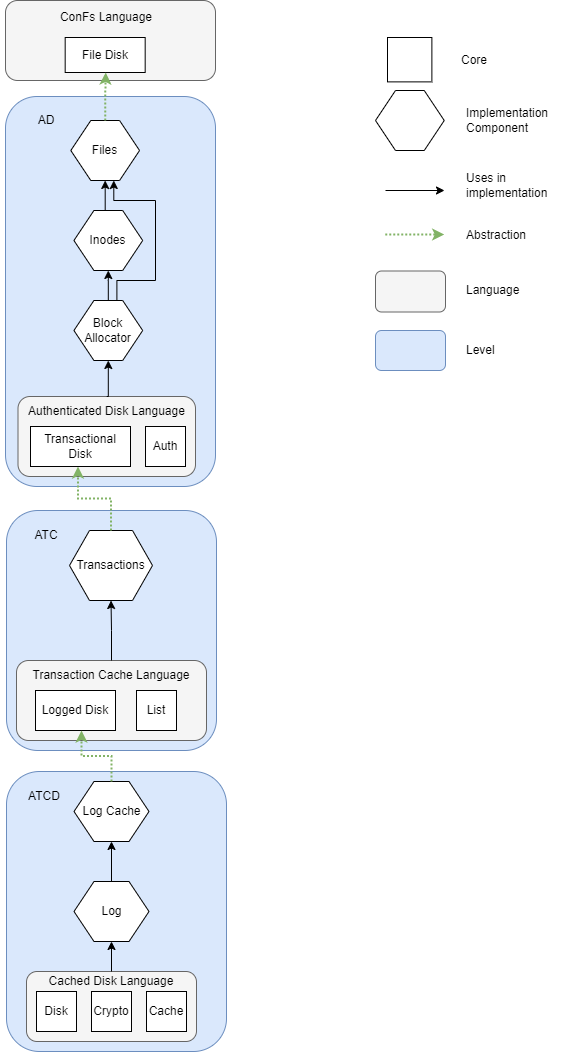
\includegraphics[scale=0.5]{templates/figures/ConFs Layers.png}
    \caption{Structure of ConFs}
    \label{fig:ConFs_Layers}
\end{figure}

\subsection{ATCD Level}
ATCD level is the lowest level of ConFs and its layer contains the model of the raw disk, a crypto engine, and in-memory data structure operations. The layer is implemented as five separate cores. These parts are disk core, crypto core, cache core, transaction list core, and the authentication core. 

Implementations in this level only uses operations from disk, crypto and cache cores; leaving transaction list and authentication cores unused. Including these cores was necessary because each file system operation will compile into a program in ATCD level and those programs will use operations from those cores. 

Thanks to the ConFrm's horizontal composition mechanism, implementations and proofs in this level uses only the relevant parts of the layer. This reduced unnecessary proof effort and implementation complexity significantly while retaining the ability to use implementations and theorems about them in the context of full level layer.

We implemented write-ahead log and log cache in this level. This level handled complicated crash and recovery semantics and presented a simple, crash-safe disk, via its representation invariant, for above levels to use. We will talk about these implementations in the following sections.


{\color{red} Table showing the state and operations of the level here}.

\subsection{ATC Level}
The level above ATCD is called ATC level and it contains a new core named logged disk that models a crash-safe disk and the possible operations on it, as well as the previously unused cores from ATCD level. ATC replaces disk, crypto, and cache cores with logged disk core. ATC also uses transaction list core, leaving authentication core unused.

Logged disk core contains an operation for each function log cache API provides. Similarly, the state of the logged disk is the crash resistant disk exposed by log cache implementation. This simplified crash semantics of the layer significantly by moving determination of possible crash states to the non-determinism tokens. This also turned its reboot and recovery semantics to a 'noop', that virtually removed the need for reasoning about the recovery process. 

\begin{figure}[H]
    \centering
\begin{verbatim}
| ExecRecover : 
      forall d u,
        exec' u Cont d Recover (Finished d tt)
        
| ExecCrashBefore :
  forall d T p u,
    exec' u CrashBefore d p (Crashed d)

| ExecCrashWriteAfter :
  forall d la lv u,
    NoDup la ->
    length la = length lv ->
    Forall (fun a => a < disk_size) la ->
    length (addr_list_to_blocks la) + length lv <= log_size ->
    exec' u CrashAfter d (Write la lv) (Crashed (upd_batch d la lv)).
\end{verbatim}
    \caption{Semantics of some of the transactional disk operations.}
    \label{fig:LD_Crash_Semantics}
\end{figure}

We implemented transactions in this level. Implementation stores active transaction in the memory as (address, block) pairs. When a transaction is committed, it deduplicates the contents based on the address - i.e. removes previous entries if an address is written multiple times in the transaction - before writing it to the log.

Implementation also enforces transaction size during a write attempt. Putting a transaction size limit allowed us to ensure that, when a transaction is committed, it will fit into the log. This design choice is made to move part of the complexity to the write function from the already complicated commit function.

{\color{red} Table showing the state and operations of the level here}.

\subsection{AD Level}
Similar to the ATC level, AD level also abstracts a part of the ATC layer. On AD level, logged disk and transaction list core is replaced with transactional disk core. ATC level's state is abstracted to a pair of disks and an indicator that stores if the transaction is empty or not. One of the disks represents the disk with active transaction applied on it. Other disk represents the disk state without the active transaction. In conjunction with transactional disk core, AD level uses authentication core to enforce access control.

Transaction being full is handled by a nondeterminism token. This abstraction allows us to remove reasoning about the precise transaction size, and turns it into a possibility that can happen in any write.

\begin{figure}[H]
    \centering
\begin{verbatim}
| ExecWrite :
  forall s a v u ,
    exec' u Cont s (Write a v) 
        (Finished (NotEmpty, ((upd (fst (snd s)) a v), snd (snd s))) (Some tt))

| ExecWriteFull :
  forall s a v u,
    exec' u TxnFull s (Write a v) 
        (Finished s None)
\end{verbatim}
    \caption{Semantics of some of the transactional disk operations.}
    \label{fig:TD_Semantics}
\end{figure}

Similar to the logged disk, if a crash happened before or after a commit is determined by a nondeterminism token. One thing to note is that rolling back to the disk without active transaction is done by the reboot function of the level.

\begin{figure}[H]
    \centering
\begin{verbatim}
| ExecCrashBefore :
  forall d T p u,
    exec' u CrashBefore d p 
        (Crashed d)

| ExecCommitCrashAfter :
  forall s u,
    exec' u CrashAfter s Commit 
        (Crashed (Empty, (fst (snd s), fst (snd s)))).
\end{verbatim}
    \caption{Transactional disk crash semantics.}
    \label{fig:TD_Crash_Semantics}
\end{figure}

Rest of the ConFs's components - i.e. block allocators, inodes and files - are implemented in this level. This level exposes the file system API.

A generic block allocator implementation is used for both inode blocks and data blocks for the files. Block allocator assumes a layout that is a single bitmap block followed by some allocatable blocks.

We implemented inodes to contain the owner of the file and a list of block numbers, which are indexes to block allocator for data blocks. There is no support for indirect blocks. ConFs stores one inode per block for simplicity.

File component uses inode functions as well as disk block allocator to implement a block based file interface. Files are represented with their inode numbers. Inode numbers are assigned by the system during file creation and returned to the user.

File component handles authentication as well as the actual manipulation of the files. Its functions are implemented as a higher-order function that handles authentication and committing or aborting, and inner functions that implements file operations.

{\color{red} Table showing the state and operations of the level here}.

\subsection{ConFs level}
ConFs level is the topmost level that provides a layer which every file system function is an operation and a state that is a mapping from inode numbers to file owner and contents. This level effectively hides all the complexities of the implementation and allows users to perceive and reason about the system similar to their intuitive understanding of it.

Inode number that is being returned upon file creation, availability of free inodes, transaction fullness, and crashes are all dictated with nondeterminism tokens.

{\color{red} Table showing the state and operations of the level here}.

% Adopted from disksec
\section{Specifiying security}
% Explains special RDNI definitions.
Security of ConFs is defined as an RDNI specification for each of the compiled FileDisk operations. In the center of these specifications is the equivalence relation between states. Since ConFs consists of four distinct levels, we had four different but related equivalence relations. We will explain these in the descending order.

\subsection{FileDisk Level Security}
We made some changes to the equivalence relation definition to unify ret\_noninterference and state\_noninterference, and to make it general enough to ensure that it can accommodate special specifications for Write and ChangeOwner operations.

We modified our equivalence relation to take an optional inode number to exclude the contents of the file that its owner is being changed.
Since equivalence relation for ChangeOwner excludes contents of the file that is being operated on, it only provides half of the required security - i.e. it excludes leakage from the changed file to the outside. The fact that no information leaks from outside to the file is covered by its functional correctness which states that file's contents stay unchanged after the operation.

\begin{figure}[H]
    \centering
\begin{verbatim}
Definition same_for_user_except (u: user) 
(exclude: option addr) (d1 d2: FD.(state)) :=
  addrs_match_exactly d1 d2 /\
  (forall inum file1 file2,
     exclude <> Some inum ->
     d1 inum = Some file1 ->
     d2 inum = Some file2 ->
     (file1.(owner) = u \/
      file2.(owner) = u) ->
     file1 = file2) /\
  (forall inum file1 file2,
     d1 inum = Some file1 ->
     d2 inum = Some file2 ->
     file1.(owner) = file2.(owner) /\ 
     length file1.(blocks) = length file2.(blocks)).
\end{verbatim}
    \caption{Equivalence relation for two FileDisk states.}
    \label{fig:eqivalence_for_filedisk}
\end{figure}


\subsection{AuthenticatedDisk and TransactionCache Level Security}
ConFrm provides a function that converts an equivalence over abstract states to an equivalence over implementation states given that a refinement between two exists. Informally, function states that two implementation states are equivalent if there exists two equivalent abstract states that are refined by the implementation states.

\begin{figure}[H]
    \centering
\begin{verbatim}
Definition refines_related 
 (related_abs:  L_abs.(state) -> L_abs.(state) -> Prop)
 (si1 si2: L_imp.(state)) : Prop :=
exists (sa1 sa2: L_abs.(state)),
  R.(refines) si1 sa1 /\
  R.(refines) si2 sa2 /\
  related_abs sa1 sa2.
\end{verbatim}
    \caption{Equivalence conversion function from ConFrm}
    \label{fig:refines_related}
\end{figure}

This function alone was sufficient derive the equivalence for these two levels. However, this is not generally is the case. Sometimes, extra conditions are needed to establish the relation between the parts of the implementation state that is abstracted away. We will present examples of such instances in the following section.

Main reason for this is that, oracles in ConFrm implicitly dictates number of execution steps a program takes. Semantics of a program requires consumption of an exactly one token per operation executed. This requirement generally implies two noninterfering programs have to follow the same execution paths. 

%%%% ADD an example noninterference spec here?

\subsection{CachedDisk Level Security}
{\color{red} INTRO HERE}

Consider the following read function:

\begin{figure}[H]
    \centering
\begin{verbatim}
Definition read a :=
  mv <- Cache_Read a;
  if mv = Some v then 
    Ret v
  else
    Disk_Read a
\end{verbatim}
    \label{fig:refines_related}
\end{figure}
%
Proving noninterference of this function requires showing that if there is an execution of the function from a state with a particular oracle, then there must be an execution from a related state with the same oracle. Since having same oracle dictates that programs have to follow the same execution paths, two related states have to contain exactly same addresses in their caches (corresponding data could be different).

If an abstraction of the states hides the existence of a cache, then refining two related abstract states is not sufficient to capture this requirement. In this instance, equivalence relation needs to be supplemented with this property to make it finer-grained.

This particular example and some other more complicated variants are present in log functions. Therefore, we supplemented the equivalence relation with the following:

{\color{red} Property here}

{\color{red} Explanation of the property here}


\section{Proving security}
We proved confidentiality of ConFs with two general categories of theorems: (1) confidentiality proofs of FileDisk operations, and (2) premises required to establish confidentiality of the refining programs of the operations. Proving (1) was relatively easy thanks to the simple structure of FileDisk state and semantics. Majority of the effort among them went into proving (2).

Proving (2) required us to prove 2 different properties for each operation: (a) oracle refinement being independent of confidential data, and (b) existence of a refined abstract oracle. Proofs in a compositional manner - i.e. corresponding properties are proved for each operation of each layer, then brought together to construct required proofs. Compositional nature of the properties significantly reduced the proof effort and repetition between layers.

One interesting case appeared regarding write operations that overwrite some data with itself. Possibility of such operations made it impossible to determine if a write succeeded or not after a crash by just examining the disk's final state. To resolve this problem, we had to reason about precise number of steps the function ran as well as the required conditions on the crash and reboot states of the disk after the execution.  This precise and low level reasoning was tedious and required significant proof effort. Despite our best efforts, question of whether this can be solved at meta-theoretic level or with another proof strategy that requires less effort remains open.

During this reasoning, we had to employ the condition that, in the log, current and residual blocks at the same address can't be identical. Encryption of each block ensured that such a condition is exponentially unlikely. By design, since a residual block and a current block cannot belong to the same transaction, they must be encrypted with different keys. Therefore such a condition does not weaken the conclusion significantly.


{\color{red} Termination Sensitivity may go here. Maybe an explanation of why it was as hard as it is?}

